\documentclass[12pt,]{article}
\usepackage{lmodern}
\usepackage{amssymb,amsmath}
\usepackage{ifxetex,ifluatex}
\usepackage{fixltx2e} % provides \textsubscript
\ifnum 0\ifxetex 1\fi\ifluatex 1\fi=0 % if pdftex
  \usepackage[T1]{fontenc}
  \usepackage[utf8]{inputenc}
\else % if luatex or xelatex
  \ifxetex
    \usepackage{mathspec}
  \else
    \usepackage{fontspec}
  \fi
  \defaultfontfeatures{Ligatures=TeX,Scale=MatchLowercase}
\fi
% use upquote if available, for straight quotes in verbatim environments
\IfFileExists{upquote.sty}{\usepackage{upquote}}{}
% use microtype if available
\IfFileExists{microtype.sty}{%
\usepackage{microtype}
\UseMicrotypeSet[protrusion]{basicmath} % disable protrusion for tt fonts
}{}
\usepackage[margin=1in]{geometry}
\usepackage[colorlinks=true,linkcolor=red,urlcolor=red,citecolor=blue]{hyperref} % cross-referencing the references and bibliography
%\usepackage{hyperref}
\PassOptionsToPackage{usenames,dvipsnames}{color} % color is loaded by hyperref
\hypersetup{unicode=true,
            pdftitle={Brief Tutorial on Documentation in R},
            colorlinks=true,
            linkcolor=blue,
            citecolor=magenta,
            urlcolor=red,
            breaklinks=true}
\urlstyle{same}  % don't use monospace font for urls
\usepackage{color}
\usepackage{fancyvrb}
\newcommand{\VerbBar}{|}
\newcommand{\VERB}{\Verb[commandchars=\\\{\}]}
\DefineVerbatimEnvironment{Highlighting}{Verbatim}{commandchars=\\\{\}}
% Add ',fontsize=\small' for more characters per line
\usepackage{framed}
\definecolor{shadecolor}{RGB}{248,248,248}
\newenvironment{Shaded}{\begin{snugshade}}{\end{snugshade}}
\newcommand{\KeywordTok}[1]{\textcolor[rgb]{0.13,0.29,0.53}{\textbf{{#1}}}}
\newcommand{\DataTypeTok}[1]{\textcolor[rgb]{0.13,0.29,0.53}{{#1}}}
\newcommand{\DecValTok}[1]{\textcolor[rgb]{0.00,0.00,0.81}{{#1}}}
\newcommand{\BaseNTok}[1]{\textcolor[rgb]{0.00,0.00,0.81}{{#1}}}
\newcommand{\FloatTok}[1]{\textcolor[rgb]{0.00,0.00,0.81}{{#1}}}
\newcommand{\ConstantTok}[1]{\textcolor[rgb]{0.00,0.00,0.00}{{#1}}}
\newcommand{\CharTok}[1]{\textcolor[rgb]{0.31,0.60,0.02}{{#1}}}
\newcommand{\SpecialCharTok}[1]{\textcolor[rgb]{0.00,0.00,0.00}{{#1}}}
\newcommand{\StringTok}[1]{\textcolor[rgb]{0.31,0.60,0.02}{{#1}}}
\newcommand{\VerbatimStringTok}[1]{\textcolor[rgb]{0.31,0.60,0.02}{{#1}}}
\newcommand{\SpecialStringTok}[1]{\textcolor[rgb]{0.31,0.60,0.02}{{#1}}}
\newcommand{\ImportTok}[1]{{#1}}
\newcommand{\CommentTok}[1]{\textcolor[rgb]{0.56,0.35,0.01}{\textit{{#1}}}}
\newcommand{\DocumentationTok}[1]{\textcolor[rgb]{0.56,0.35,0.01}{\textbf{\textit{{#1}}}}}
\newcommand{\AnnotationTok}[1]{\textcolor[rgb]{0.56,0.35,0.01}{\textbf{\textit{{#1}}}}}
\newcommand{\CommentVarTok}[1]{\textcolor[rgb]{0.56,0.35,0.01}{\textbf{\textit{{#1}}}}}
\newcommand{\OtherTok}[1]{\textcolor[rgb]{0.56,0.35,0.01}{{#1}}}
\newcommand{\FunctionTok}[1]{\textcolor[rgb]{0.00,0.00,0.00}{{#1}}}
\newcommand{\VariableTok}[1]{\textcolor[rgb]{0.00,0.00,0.00}{{#1}}}
\newcommand{\ControlFlowTok}[1]{\textcolor[rgb]{0.13,0.29,0.53}{\textbf{{#1}}}}
\newcommand{\OperatorTok}[1]{\textcolor[rgb]{0.81,0.36,0.00}{\textbf{{#1}}}}
\newcommand{\BuiltInTok}[1]{{#1}}
\newcommand{\ExtensionTok}[1]{{#1}}
\newcommand{\PreprocessorTok}[1]{\textcolor[rgb]{0.56,0.35,0.01}{\textit{{#1}}}}
\newcommand{\AttributeTok}[1]{\textcolor[rgb]{0.77,0.63,0.00}{{#1}}}
\newcommand{\RegionMarkerTok}[1]{{#1}}
\newcommand{\InformationTok}[1]{\textcolor[rgb]{0.56,0.35,0.01}{\textbf{\textit{{#1}}}}}
\newcommand{\WarningTok}[1]{\textcolor[rgb]{0.56,0.35,0.01}{\textbf{\textit{{#1}}}}}
\newcommand{\AlertTok}[1]{\textcolor[rgb]{0.94,0.16,0.16}{{#1}}}
\newcommand{\ErrorTok}[1]{\textcolor[rgb]{0.64,0.00,0.00}{\textbf{{#1}}}}
\newcommand{\NormalTok}[1]{{#1}}
\usepackage{longtable,booktabs}
\usepackage{graphicx,grffile}
\makeatletter
\def\maxwidth{\ifdim\Gin@nat@width>\linewidth\linewidth\else\Gin@nat@width\fi}
\def\maxheight{\ifdim\Gin@nat@height>\textheight\textheight\else\Gin@nat@height\fi}
\makeatother
% Scale images if necessary, so that they will not overflow the page
% margins by default, and it is still possible to overwrite the defaults
% using explicit options in \includegraphics[width, height, ...]{}
\setkeys{Gin}{width=\maxwidth,height=\maxheight,keepaspectratio}
\IfFileExists{parskip.sty}{%
\usepackage{parskip}
}{% else
\setlength{\parindent}{0pt}
\setlength{\parskip}{6pt plus 2pt minus 1pt}
}
\setlength{\emergencystretch}{3em}  % prevent overfull lines
\providecommand{\tightlist}{%
  \setlength{\itemsep}{0pt}\setlength{\parskip}{0pt}}
\setcounter{secnumdepth}{5}
% Redefines (sub)paragraphs to behave more like sections
\ifx\paragraph\undefined\else
\let\oldparagraph\paragraph
\renewcommand{\paragraph}[1]{\oldparagraph{#1}\mbox{}}
\fi
\ifx\subparagraph\undefined\else
\let\oldsubparagraph\subparagraph
\renewcommand{\subparagraph}[1]{\oldsubparagraph{#1}\mbox{}}
\fi

%%% Use protect on footnotes to avoid problems with footnotes in titles
\let\rmarkdownfootnote\footnote%
\def\footnote{\protect\rmarkdownfootnote}

%%% Change title format to be more compact
\usepackage{titling}

% Create subtitle command for use in maketitle
\newcommand{\subtitle}[1]{
  \posttitle{
    \begin{center}\large#1\end{center}
    }
}

\setlength{\droptitle}{-2em}

  \title{Brief Tutorial on Documentation in R}
    \pretitle{\vspace{\droptitle}\centering\huge}
  \posttitle{\par}
    \author{}
    \preauthor{}\postauthor{}
    \date{}
    \predate{}\postdate{}
  
\linespread{1.25}

\begin{document}
\maketitle

{
\hypersetup{linkcolor=black}
\setcounter{tocdepth}{2}
\tableofcontents
}
A \# followed by text becomes your title!

\section{Brief tutorial on R
Manrkdown}\label{brief-tutorial-on-r-manrkdown}

Optional YAML metadata resides between two tripple dashes:
\texttt{-\/-\/-}

Section begins by two hashes: \#\#

\subsection{Section 1}\label{section-1}

This is goign to be a first document.

How do we include an R code in this doc? Well just press: Ctrl-Alt-I and
a code separator (three back ticks: ```) will appear!

\begin{Shaded}
\begin{Highlighting}[]
\KeywordTok{require}\NormalTok{(dplyr);}
\NormalTok{ns =}\StringTok{ }\NormalTok{dplyr::nasa;}
\NormalTok{ns =}\StringTok{ }\KeywordTok{as.data.frame}\NormalTok{(ns);}
\NormalTok{mean_lat =}\StringTok{ }\KeywordTok{mean}\NormalTok{(ns$lat, }\DataTypeTok{na.rm =} \NormalTok{T);}
\NormalTok{mean_lat}
\end{Highlighting}
\end{Shaded}

\begin{verbatim}
## [1] 7.5
\end{verbatim}

But I dont want to see all these messages in my doc. I am going to run
the above with option: \texttt{include\ =\ FALSE}

See nothing got printed above!

But I do want to display the output but not the code! Use
\texttt{echo\ =\ FALSE} instead.

\begin{verbatim}
## [1] 7.5
\end{verbatim}

Now only the output got printed. This is what I really wanted!

What if I wanted to dynamically use a value in my doc? Like generated
from a computation? We can do that by writing within backticks with
first letter being \texttt{r}. So mean latitude is 7.5. This makes it
very easy to update report in future with minimal changes. Lets write
counting from 1 to 10: 1, 2, 3, 4, 5, 6, 7, 8, 9, 10

Now, let's make a plot!

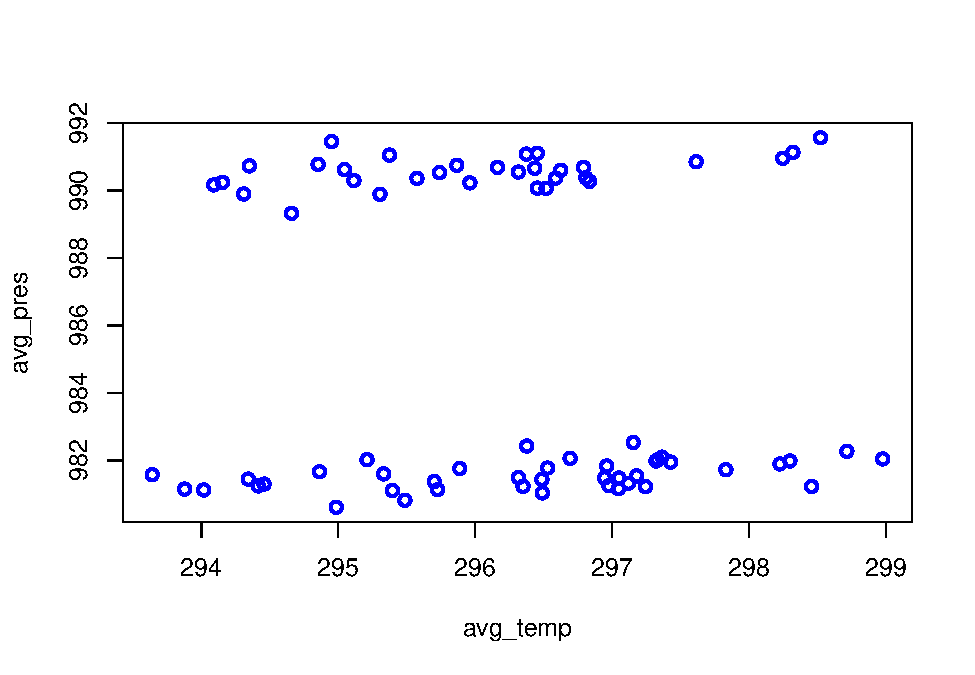
\includegraphics{first_doc_files/figure-latex/unnamed-chunk-4-1.pdf}

The plot here is a bit too big. I would like a smaller one for my doc:

\begin{figure}[htbp]
\centering
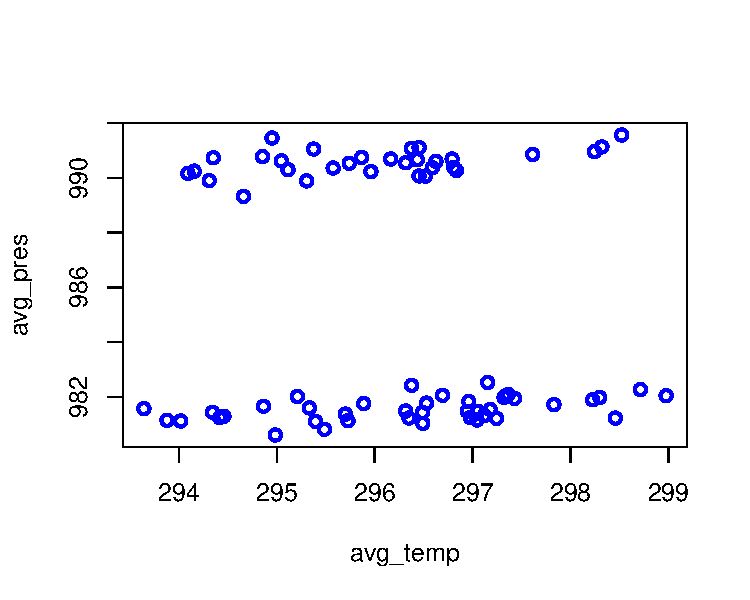
\includegraphics{first_doc_files/figure-latex/unnamed-chunk-5-1.pdf}
\caption{avg pressure vs avg temp}
\end{figure}

See the above fits much better!

\subsection{Section 2}\label{section-2}

To get code within the doc (in teletype constant width fonts), use
single backtics: \texttt{code}, Package \texttt{dplyr}

Block quote begins with \texttt{\textgreater{}} sign:

\begin{quote}
This is a block quote!
\end{quote}

Any text within a pair of \texttt{*} is \texttt{*italicized*}:
\emph{italicized} and within \texttt{**} is \texttt{**bolded**}:
\textbf{bolded}

Single star followed by a space: \texttt{*} produces bullet points! 4
blank spaces, a star and then a space:
\texttt{\textbar{}\ \ \ \ *\ \textbar{}} produces sub-itmes! It can be
further generalized!

\begin{itemize}
\tightlist
\item
  1
\item
  2

  \begin{itemize}
  \tightlist
  \item
    2.1
  \item
    2.2

    \begin{itemize}
    \tightlist
    \item
      2.2.1
    \end{itemize}
  \end{itemize}
\end{itemize}

\subsection{Section 3}\label{section-3}

Math mode can be entered by writing everything within pair of dollar
signs: \texttt{\$}.

\(F = m \cdot a\), \(\lambda^2 \gamma\), \(\infty\), and so on!

Write a block of equations using two dollar signs instead of one:
\texttt{\$\$}. \[\int e^x dx = e^x + C\].

Use underscore \texttt{\_} for subscripts and exponent \texttt{\^{}} for
superscript. \texttt{H\_0} is \(H_0\) and \texttt{H\^{}0} is \(H^0\).
Use curly brackets to combine parts of an equation, i.e.~to write
\texttt{lambda\^{}(a+b)} as \texttt{\textbackslash{}lambda\^{}\{a+b\}}:
\(\lambda^{a+b}\)

\subsection{Section 4}\label{section-4}

Use extra hash \texttt{\#} for sub-sectioning.

\subsubsection{Sub-section 4.1}\label{sub-section-4.1}

\subsubsection{Sub-sub-section 4.1.1}\label{sub-sub-section-4.1.1}

\subsubsection{Sub-sub-sub-section
4.1.1.1}\label{sub-sub-sub-section-4.1.1.1}

\subsubsection{Sub-sub-sub-sub-section
4.1.1.1.1}\label{sub-sub-sub-sub-section-4.1.1.1.1}

\subsection{Section 5}\label{section-5}

To create a document, a process called knitting, you can simply click to
knit on Rmarkdown interface. Or, you can incoke the command line:
\texttt{rmarkdown::render("first\_doc.Rmd")}

\subsection{Section 6}\label{section-6}

Hyperlink can be added by writing text within braces \texttt{{[}{]}}
followed by the weblink written within parantheses \texttt{()}. Thus you
write like: \texttt{{[}Google{]}(https://www.google.com/)} to get
\href{https://www.google.com/}{Google}.

Footnote can be added by \texttt{{[}\^{}1{]}}. Here is one.\footnote{That's
  my foot note!}

You can also add a reference using \texttt{{[}@bib\_ref{]}}. For
instance I'll make a reference here: (Baumer et al.
\protect\hyperlink{ref-baumer2014r}{2014}). Also don't forget to add a
section on References and mention the \texttt{.bib} file in YAML
metadata.

\subsection{Section 7}\label{section-7}

Let's make a table. Use the \texttt{result\ =\ "asis"} option to make
sure that the table output is processed as is and not further processed!

\% Table created by stargazer v.5.2 by Marek Hlavac, Harvard University.
E-mail: hlavac at fas.harvard.edu \% Date and time: Tue, Jun 26, 2018 -
02:19:00 PM

\begin{table}[!htbp] \centering 
  \caption{Table with Stargazer in Rmarkdown} 
  \label{} 
\begin{tabular}{@{\extracolsep{5pt}}lc} 
\\[-1.8ex]\hline 
\hline \\[-1.8ex] 
 & \multicolumn{1}{c}{\textit{Dependent variable:}} \\ 
\cline{2-2} 
\\[-1.8ex] & y \\ 
\hline \\[-1.8ex] 
 x & 0.981$^{***}$ \\ 
  & (0.017) \\ 
  & \\ 
 Constant & 0.002 \\ 
  & (0.016) \\ 
  & \\ 
\hline \\[-1.8ex] 
Observations & 1,000 \\ 
R$^{2}$ & 0.778 \\ 
Adjusted R$^{2}$ & 0.778 \\ 
Residual Std. Error & 0.515 (df = 998) \\ 
F Statistic & 3,497.193$^{***}$ (df = 1; 998) \\ 
\hline 
\hline \\[-1.8ex] 
\textit{Note:}  & \multicolumn{1}{r}{$^{*}$p$<$0.1; $^{**}$p$<$0.05; $^{***}$p$<$0.01} \\ 
\end{tabular} 
\end{table}

\subsection{Section 8}\label{section-8}

Let's make table:

\begin{longtable}[]{@{}lcr@{}}
\caption{Your Caption}\tabularnewline
\toprule
First Header & Second Header & Third Header\tabularnewline
\midrule
\endfirsthead
\toprule
First Header & Second Header & Third Header\tabularnewline
\midrule
\endhead
First row & Data & Very long data entry\tabularnewline
Second row & \textbf{Cell} & \emph{Cell}\tabularnewline
Third row & Cell that spans across two columns &\tabularnewline
\bottomrule
\end{longtable}

\subsection{Section 9}\label{section-9}

\begin{equation}
a=b^2
\end{equation}

\section*{References}\label{references}
\addcontentsline{toc}{section}{References}

\hypertarget{refs}{}
\hypertarget{ref-baumer2014r}{}
Baumer, Ben, Mine Cetinkaya-Rundel, Andrew Bray, Linda Loi, and Nicholas
J Horton. 2014. ``R Markdown: Integrating a Reproducible Analysis Tool
into Introductory Statistics.'' \emph{ArXiv Preprint ArXiv:1402.1894}.


\end{document}
